% https://tex.stackexchange.com/questions/387047/the-duck-pond-showcase-of-tikz-drawn-animals-ducks/420405#420405
\documentclass{article}
\usepackage{animate}
\usepackage{xsavebox}
\usepackage{tikzducks}
\usepackage{graphicx}
\usetikzlibrary{shapes.callouts,calc}

%%%%%%%%%%%%%%%%%%%%%%%%%%%%%%%%%%%%%%%
%% adjustable parameter: frame number; 
%% enlarge for smoothness 
\newcommand\framefac{2} % times 72
%%%%%%%%%%%%%%%%%%%%%%%%%%%%%%%%%%%%%%%

%%%%%%%%%%%%%%%%%%%%%%%%%%%%%%%%%%%%%%%%%%%%%%%%%%%%%%%%%%%%%
%% uncomment this section to export animation
%% to multipage PDF a.pdf and run
%% 
%%  convert -density 300 -delay 4 -loop 0 -alpha remove a.pdf b.gif
%%
%% to get an animated GIF b.gif at 100/4 = 25 frames per s
%%%%%%%%%%%%%%%%%%%%%%%%%%%%%%%%%%%%%%%%%%%%%%%%%%%%%%%%%%%%%
%\usepackage[active,tightpage]{preview}
%\makeatletter
%\def\@anim@@newframe{\@ifstar\@anim@newframe\@anim@newframe}
%\def\@anim@newframe{\end{preview}\begin{preview}}
%\renewenvironment{animateinline}[2][]{%
%\let\newframe\@anim@@newframe%
%\let\multiframe\@anim@multiframe%
%\begin{preview}}{%
%\end{preview}}
%\makeatother
%%%%%%%%%%%%%%%%%%%%%%%%%%%%%%%%%%%%%%%%%%%%%%%%%%%%%%%%%%%%%

\newcommand\DuckSong[1]{\ifcase#1
All%
\or
my%
\or
little%
\or
ducklings,%
\or
Swimming%
\or
in%
\or
the%
\or
lake,%
\or
Heads%
\or
dunk%
\or
in%
\or
the%
\or
water,%
\or
As%
\or
little%
\or
tails%
\or
do%
\or
shake.%
\fi%
}

\ExplSyntaxOn
\let\intEval\int_eval:n
\let\intMod\int_mod:nn
\let\intComp\int_compare:nTF
\let\intCase\int_case:nnF
\ExplSyntaxOff

\begin{document}

\xsbox{Duck}{\tikz{\duck}}%
\xsbox{CarlaDuck}{\tikz{\duck[pizza,squareglasses=brown!50!black,longhair=black!70!brown]}}%
\xsbox{Boat}{\tikz{%
  \filldraw[fill=white,line width=0.1pt] (0.6,0.71)--(1,1.2)--(1.4,0.71)--(1,0.6)--cycle;
  \node[scale=0.1,rotate=10,anchor=south east] at (2.3,0.9) {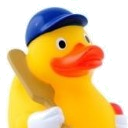
\includegraphics{pauloTransp}};
  \filldraw[fill=white,line width=0.1pt] (0,0)--(2,0)--(2.4,1)--(1,0.6)--(-0.4,1)--cycle;}}%
\begin{animateinline}[autoplay, loop, controls=false]{25}
  \multiframe{\intEval{72*\framefac}}{iX=0+1}{
  \begin{tikzpicture}
    \fill[use as bounding box,white!90!blue] (-1,-1) rectangle (7.2,3);
    \node[scale=2,anchor=center,rotate=6*cos(360/(72*\framefac-1)*\iX)] at ({-3.8+\iX*13.8/(72*\framefac-1)},{0.9+0.1*sin(360/(72*\framefac-1)*\iX)}){\theBoat};
    \fill[blue!60!black] plot[variable=\x,domain=-1:7.2,samples=82] ({\x},{0.1+0.3*sin(100*(\x-0.5*\iX/10/\framefac))})--(7.2,-1)--(-1,-1)--(-1,0);
    \fill[blue] plot[variable=\x,domain=-1:7.2,samples=82] ({\x},{0.05+0.3*sin(100*(\x-\iX/10/\framefac))})--(7.2,-1)--(-1,-1)--(-1,0);
    \node[rotate=27.63*cos(100*(2.2-\iX/10/\framefac))] (duck) at ({2.2},{0.95+0.3*sin(100*(2.2-\iX/10/\framefac))}){\theCarlaDuck};
    \node[ellipse callout,text width=3.5em,align=center,draw,anchor=east,callout absolute pointer={($(duck.west)+(0.3,0.1)$)},fill=white] (song)
      at ($(duck)+(-1,1)$) {\makebox[0pt][c]{\DuckSong{\intEval{(\iX-\intMod{\iX}{4*\framefac})/(4*\framefac)}}}};
    \foreach \duckscal/\duckoff in {0.3/0,0.25/1,0.2/2,0.15/3,0.12/4}  
      \node[
        rotate=\intComp{\duckoff<4}{0}{\intComp{\iX<36*\framefac}{0}{
        \intCase{\iX}{{36*\framefac}{22.5}{36*\framefac+1}{45}{36*\framefac+2}{67.5}{72*\framefac-3}{67.5}{72*\framefac-2}{45}{72*\framefac-1}{22.5}}{90}}}
        +27.63*cos(100*(3.6+\duckoff*0.7-\iX/10/\framefac)),scale=\duckscal,anchor=south] at ({3.6+\duckoff*0.7},{0.3*sin(100*(3.6+\duckoff*0.7-\iX/10/\framefac))-0.04}){\theDuck};
    \fill[blue] plot[variable=\x,domain=-1:7.2,samples=82] ({\x},{0.3*sin(100*(\x-\iX/10/\framefac))})--(7.2,-1)--(-1,-1)--(-1,0);
    \fill[blue!60!white] plot[variable=\x,domain=-1:7.2,samples=82] ({\x},{0.3*sin(100*(\x-2*\iX/10/\framefac))-0.2})--(7.2,-1)--(-1,-1)--(-1,0);
    \draw[white,line width=1pt] (-1,-1) rectangle (7.2,3);
  \end{tikzpicture}
  }
\end{animateinline}

\end{document}